%% Exemplo de utilizacao do estilo de formatacao abnt-UTFPR.cls para LaTeX (v1.3)
%% Autores: Hugo Vieira Neto (hvieir@utfpr.edu.br)
%%          Diogo Rosa Kuiaski (diogo.kuiaski@gmail.com)

\documentclass{abnt-UTFPR} % estilo de documento abnTeX
\usepackage[alf,abnt-emphasize=bf,bibjustif,recuo=0cm]{abntcite} % estilo de bibliografia abnTeX
\usepackage[brazil]{babel} % pacote portugues brasileiro
%\usepackage[latin1]{inputenc} % pacote para acentuacao direta
\usepackage{amsmath,amsfonts,amssymb} % pacote matematico
\usepackage{graphicx} % pacote grafico


% ---------- Preambulo ----------
\instituicao{Universidade Tecnol\'ogica Federal do Paran\'a} % nome da instituicao
\departamento{Departamento Acad\^emico de Eletr\^onica} % nome do departamento
\programa{Curso de Engenharia da Computa\c{c}\~ao} % nome do curso

\documento{Trabalho Acad\^emico} % tipo de documento
\unidade{Oficina de Integra\c{c}\~ao II} % unidade curricular

\titulo{Interface de Instrumento Musical Eletr\^onico} % titulo do trabalho em portugues
\title{Electronic Musical Instrument Interface} % titulo do trabalho em ingles

\autor{Felipe Luiz Bill} % primeiro autor do trabalho
\autordois{Felipe Michels Fontoura} % segundo autor do trabalho, caso exista
\autortres{Leandro Piekarski do Nascimento} % terceiro autor do trabalho, caso exista
\autorquatro{Lucio Eiji Assaoka Hossaka} % quarto autor do trabalho, caso exista
\cita{BILL, Felipe; Nascimento, Leandro do; FONTOURA, Felipe; HOSSAKA, Lucio} % sobrenome (maiusculas) e nome do(s) autor(es) do trabalho, separados por ponto-e-virgula (ate quatro autores para trabalhos de unidades curriculares)

\palavraschave{Instrumento Musical, Sintetizador} % palavras-chave do trabalho
\keywords{Musical Instrument, Synthesizer} % palavras-chave do trabalho em ingles

\comentario{\UTFPRdocumentodata\ apresentado \`a Unidade Curricular de \UTFPRunidadedata\ do \UTFPRprogramadata\ da \ABNTinstituicaodata\ como requisito parcial para aprova\c{c}\~ao.}

\orientador{Prof. Dr. Miguel Antonio Sovierzoski. } % nome do orientador do trabalho
%\orientador[Orientadora:]{Nome da Orientadora} % <- no caso de orientadora, usar esta sintaxe
%\coorientador{Nome do Co-orientador} % nome do co-orientador do trabalho, caso exista
%\coorientador[Co-orientadora:]{Nome da Co-orientadora} % <- no caso de co-orientadora, usar esta sintaxe

\local{Curitiba} % cidade
\data{2009} % ano


%---------- Inicio do Documento ----------
\begin{document}

\capa % geracao automatica da capa
\folhaderosto % geracao automatica da folha de rosto
%\termodeaprovacao % <- ainda a ser implementado corretamente


% epigrafe (opcional)
\begin{epigrafe}
Se voc\^e tem uma ma\c{c}\~a e eu tenho uma ma\c{c}\~a, e n\'os trocamos as ma\c{c}\~as, n\'os, ambos, continuamos a ter apenas uma ma\c{c}\~a. Contudo se voc\^e tem uma id\'eia e eu tenho uma id\'eia, e n\'os trocamos as id\'eias, cada um de n\'os agora tem duas id\'eias. (SHAW, George Bernard).
\end{epigrafe}

%resumo
\begin{resumo}
Este trabalho apresenta, com detalhamento pr\'atico e te\'orico, o projeto de uma interface humano-m\'aquina que simula um instrumento musical de cordas. Faz-se uma breve explana\c{c}\~ao acerca do hist\'orico dos instrumentos eletr\^onicos e do funcionamento dos instrumentos musicais de corda. Exp\~oe-se em detalhes os aspectos t\'ecnicos do hardware utilizado, e em seguida lista os independentemente os componentes de hardware e de software envolvidos na execu\c{c}\~ao da interface. Finaliza-se com uma avalia\c{c}\~ao da relev\^ancia do projeto atrav\'es da discuss\~ao de suas aplica\c{c}\~oes. Este trabalho \'e complementado pela an\'alise do projeto, do ponto de vista da metodologia da pesquisa, apresentando considera\c{c}\~oes sobre a arquitetura do sistema, implementa\c{c}\~ao, testes, valida\c{c}\~ao, gerenciamento de riscos, cronograma, or\c{c}amento e pessoal. Traz como resultado uma das muitas possibilidades inexploradas na perspectiva do uso da tecnologia no meio musical e art\'istico.
\end{resumo}

%abstract
\begin{abstract}
This paper presents, with theoretical and practical details, the design of a human-machine interface that simulates a string musical instrument. 

It makes a brief explanation about the history of electronic instruments and the operation of string musical instruments. Exposes in detail the technical aspects of the hardware used, and then lists the independent components of hardware and software involved in the implementation of the interface. 

It finishes with an assessment of the relevance of the project by discussing its applications. This work is complemented by the analysis of the project, in terms of research method, with respect to system architecture, implementation, testing, validation, risk management, schedule, budget and staff. As a result, it brings a new possibility  when it comes to artistic and musical expression through technology.
\end{abstract}

% listas (opcionais, mas recomenda-se a partir de 5 elementos)
\listadefiguras % geracao automatica da lista de figuras
\listadetabelas % geracao automatica da lista de tabelas

% sumario
\sumario % geracao automatica do sumario


%---------- Inicio do Texto ----------
% recomenda-se a escrita de cada capitulo em um arquivo texto separado (exemplo: intro.tex, fund.tex, exper.tex, concl.tex, etc.) e a posterior inclusao dos mesmos no mestre do documento utilizando o comando \input{}, da seguinte forma:
%\input{intro.tex}
%\input{fund.tex}
%\input{exper.tex}
%\input{concl.tex}


%---------- Primeiro Capitulo ----------
\chapter{Introdu\c{c}\~ao}

Na d\'ecada de 70, um grupo de fabricantes de instrumentos musicais desenvolveu um padr\~ao de mensagens de controle entre instrumentos musicais, o padr\~ao MIDI (Musical Instrument Digital Interface). Essas mensagens n\~ao cont\^em o \'audio propriamente dito, mas instru\c{c}\~oes protocoladas, que definem notas, timbre, ritmo e efeitos usados por sintetizadores para produzir som.

Seguindo o caminho inverso, recentemente, surgiram interfaces eletr\^onicas que simulam instrumentos musicais. Popularizadas pela s\'erie de jogos ``Guitar Hero'', guitarras, baterias e outros instrumentos s\~ao simulados. Essas interfaces recebem entradas de dados atrav\'es de bot\~oes e as convertem em instru\c{c}\~oes que s\~ao interpretadas por um software. Por sua vez, o software gera o \'audio, de acordo com as entradas.

Em um esfor\c{c}o semelhante, um instrumento musical eletr\^onico foi criado: o traut\^onio. Vale ressaltar que sua inven\c{c}\~ao foi realizada muito antes dos eventos acima descritos.  Concebido por Friedrich Trautwein, em 1929, logo atraiu m\'usicos como, mais notadamente, Oskar Sala, que construiu suas pr\'oprias vers\~oes do instrumento. Em suma, o aparelho \'e composto por um fio resistivo, que varia sua diferen\c{c}a de potencial (ddp) conforme \'e tocado. A ddp serve como entrada para o sintetizador, que a converte em emiss\~ao sonora.

O projeto desenvolvido consiste em uma interface eletr\^onica, cujo funcionamento \'e semelhante ao do traut\^onio. Todavia, o projeto \'e composto por mais de uma corda, e n\~ao apresenta sintetizador.

\section{Motiva\c{c}\~ao}

Com o desenvolvimento da tecnologia ap\'os a Terceira Revolu\c{c}\~ao Industrial - nomenclatura considerada discut\'ivel por alguns historiadores, por\'em facilmente compreensivel sobre a que se refere -, existe atualmente a forte tend\^encia de se integrar computa\c{c}\~ao, rob\'otica e eletr\^onica em diversos setores da sociedade, al\'em da habitual aplica\c{c}\~ao industrial dessas tecnologias. 

Um  dos setores em que o amparo tecnol\'ogico mais se destaca \'e o da m\'usica. N\~ao somente no que se refere \`a grava\c{c}\~ao e armazenamento, mas, em especial, no que se refere \`a composi\c{c}\~ao. Atualmente, existem ferramentas que permitem at\'e mesmo confec\c{c}\~ao de partituras com sintetiza\c{c}\~ao sonora. 

Esta proposta \'e um esfor\c{c}o no sentido de prover um instrumento musical eletr\^onico que permita tamb\'em, entre outras fun\c{c}\~oes, a representa\c{c}\~ao musical atrav\'es de recursos de v\'ideo. Ela foi motivada pelo interesse comum dos integrantes da equipe de desenvolvimento pela m\'usica e pelo design de intera\c{c}\~ao. 

\section{Objetivos}

\subsection{Objetivos Gerais}

Criar um prot\'otipo de um instrumento musical eletr\^onico de cordas e desenvolver um software que receba e interprete os sinais enviados por um circuito el\'etrico, sendo esse respons\'avel pela interface de intera\c{c}\~ao com o usu\'ario. 

\subsection{Objetivos Espec\'ificos}

Aprimorar conhecimentos em:
\begin{itemize} 
\item Eletr\^onica anal\'ogica, eletr\^onica digital, convers\~ao anal\'ogico-digital;
\item Intera\c{c}\~ao hardware-software, sensores;
\item Trabalho entre equipes multidisciplinares;
\item No\c{c}\~oes de metodologia da pesquisa;
\item No\c{c}\~oes de gerenciamento de projetos, testes e no\c{c}\~oes de gerenciamento de prazos.
\end{itemize}

Aplicar conhecimentos e esfor\c{c}os condizentes para desenvolver as bases de um projeto posterior de instrumento musical.

\section{Princ\'ipio de Funcionamento dos Instrumentos de Corda}

Os instrumentos de cordas apresentam cordas tensionadas, sob a\c{c}\~ao de algum tipo de for\c{c}a, o que faz com que oscilem, produzindo sons. \'E comum classificar esses instrumentos de acordo com a forma como a corda \'e percutida. Os instrumentos de cordas friccionadas s\~ao tocados por fric\c{c}\~ao sobre as cordas, normalmente usando um arco, como \'e o caso do violino ou do violoncelo. Os instrumentos de cordas beliscadas s\~ao tocados por belisc\~oes ou empurr\~oes tangentes \`as cordas, como \'e o caso do viol\~ao e do cravo. Os instrumentos de cordas percutidas s\~ao tocados por impacto sobre as cordas, como \'e o caso do piano.

Alguns instrumentos de cordas friccionadas ou beliscadas apresentam as cordas dispostas numa parte do instrumento denominada ``bra\c{c}o''. Em tais instrumentos, as cordas s\~ao pressionadas pelo instrumentista em determinados pontos do bra\c{c}o, de forma que a corda s\'o oscile a partir do ponto em que foi pressionada, o que define a altura (tonalidade) do som. A forma em que o impacto, o belisco ou a fric\c{c}\~ao s\~ao produzidos define a intensidade (volume) do som. S\~ao exemplos instrumentos como o viol\~ao, o violino e o violoncelo. Do ponto de vista t\'ecnico, pode-se dizer que tais instrumentos recebem dois ``par\^ametros'' ou ``sinais de entrada'' para cada uma das cordas: o ``toque'', ou seja, a oscila\c{c}\~ao ou n\~ao da corda, e a posi\c{c}\~ao do dedo no bra\c{c}o. Em contrapartida, o instrumento envia uma ``resposta'' ou ``sinal de sa\'ida'': o som na frequ\^encia, no timbre e na intensidade desejados.

� medida em que a posi\c{c}\~ao em que a corda � pressionada pelo dedo do instrumentista for mais distante da extremidade mais externa do bra\c{c}o do instrumento, a parte oscilante da corda diminui, e a frequ\^encia sonora gerada aumenta. Essa varia\c{c}\~ao n\~ao \'e linear, e tampouco o \'e a percep\c{c}\~ao dessa frequ\^encia pelo ouvido humano. Reduzindo-se o comprimento oscilante da corda pela metade, aumenta-se uma oitava, ou seja, toca-se a mesma nota mais aguda.

\'E poss\'ivel estabelecer uma rela\c{c}\~ao entre a posi\c{c}\~ao em que o dedo \'e pressionado numa corda (a partir da extremidade mais externa do bra\c{c}o) e a frequ\^encia gerada ao percutir tal corda. Na f\'ormula apresentada pela equa\c{c}\~ao \ref{eq:freq}, o tamanho do trecho tensionado das cordas \'e representado por $L$, e a frequ\^encia do harm\^onico fundamental da corda, ou seja, aquela que \'e produzida ao toc\'a-la sem pressionar (matematicamente equivalente a pression\'a-lo na extremidade  o ponto $0$) \'e representada por $f_0$.

\begin{equation}
f(x) = f_0*{{L-x}/L}
\label{eq:freq}
\end{equation}

Supondo um instrumento com uma \'unica corda, com comprimento de um metro e afinada em d\'o (com frequ\^encia 523,25 Hz), tem-se o gr\'afico de frequ\^encia por posi\c{c}\~ao exibido na figura~\ref{fig:graficofrequencia}.

\begin{figure}[!htb]
	\centering
	\includegraphics[scale = 0.5]{./figs/graficofreq.eps} % <- formatos PNG, JPG e PDF
	\caption[Gr\'afico em Excel da Frequ\^encia vs. Posi\c{c}\~ao]{Gr\'afico de Frequ\^encia por Posi\c{c}\~ao de um instrumento de corda fict\'icio.}
	\fonte{Autoria Pr\'opria}
	\label{fig:graficofrequencia}
\end{figure}

Os pontos em destaque no gr\'afico apresentado na figura \ref{fig:graficofrequencia} s\~ao as notas da escala diat\^onica maior (a mesma escala representada pelas teclas brancas do piano). O gr\'afico apresenta apenas tr\^es oitavas, ou seja, tr\^es trechos de d\'o a d\'o. Na tabela~\ref{tab:freq} est\~ao apresentados os valores correspondentes de nota, posi\c{c}\~ao e frequ\^encia:

\begin{table}[!htb]
	\centering
	\caption[Frequ\^encias das Notas Musicais da Escala Diat\^onica]{Frequ\^encias das Notas Musicais da Escala Diat\^onica}
	\label{tab:freq}
	\begin{tabular}{ccc}
\hline
Nota & Posi\c{c}\~ao (cm) & Frequ\^encia (Hz) \\
\hline
d\'o & 0,00 & 523,25 \\
r\'e & 10,91 & 587,33 \\
mi & 20,63 & 659,26 \\
f\'a & 25,08 & 698,46 \\
sol & 33,26 & 784,00 \\
l\'a & 40,54 & 880,00 \\
si & 47,03 & 987,77 \\
d\'o & 50,00 & 1046,50 \\
r\'e & 55,46 & 1174,66 \\
mi & 60,31 & 1318,51 \\
f\'a & 62,54 & 1396,91 \\
sol & 66,63 & 1567,98 \\
l\'a & 70,27 & 1760,00 \\
si & 73,51 & 1975,53 \\
d\'o & 75,00 & 2093,01 \\
r\'e & 77,73 & 2349,32 \\
mi & 80,16 & 2637,02 \\
f\'a & 81,27 & 2793,83 \\
sol & 83,31 & 3135,96 \\
l\'a & 85,13 & 3520,00 \\
si & 86,76 & 3951,07 \\
d\'o & 87,50 & 4186,01 \\
\hline
	\end{tabular}
	\fonte{Autoria pr\'opria.}
\end{table}

O instrumento fict\'icio apresentado acima tem uma fun\c{c}\~ao frequ\^encia/posi\c{c}\~ao cont\'inua. Em contrapartida a essa forma de resposta da frequ\^encia, alguns outros instrumentos possuem uma fun\c{c}\~ao frequ\^encia/posi\c{c}\~ao discreta, comumente atrav\'es do uso de trastes, pequenos peda\c{c}os de metal que demarcam a ``zona'' do bra\c{c}o em que se pressiona para produzir cada nota. Um exemplo de instrumento com fun\c{c}\~ao de frequ\^encia cont\'inua \'e o violino, e um exemplo de instrumento com fun\c{c}\~ao de frequ\^encia discreta \'e o viol\~ao. O projeto descrito neste trabalho \'e um sistema de entrada de dados cuja forma de utiliza\c{c}\~ao, do ponto de vista do usu\'ario, \'e semelhante \`a de um instrumento de frequ\^encia discreta, especialmente do viol\~ao e da guitarra el\'etrica.


%---------- Segundo Capitulo ----------
\chapter{Proposta}
\label{chap:proposta}

A especifica\c{c}\~ao de um produto a ser desenvolvido pode ser dividida em tr\^es partes: os requisitos funcionais, os requisitos n\~ao-funcionais, e os requisitos de dom\'inio. Os requisitos funcionais s\~ao aqueles que definem o objetivo e a opera\c{c}\~ao do artefato. Os requisitos n\~ao-funcionais s\~ao as propriedades emergentes do sistema, como: desempenho, confiabilidade, facilidade de manuten\c{c}\~ao ou usabilidade.

Para esta proposta os requisitos funcionais s\~ao:

\begin{itemize}
\item Uma interface (f\'isica) de um instrumento musical, composta por uma ou mais cordas. As cordas s\~ao fios resistivos, que variam a tens\~ao do circuito el\'etrico conforme a posi\c{c}\~ao em que s\~ao pressionadas. Essa tens\~ao \'e passada a um interpretador/sintetizador de som;
\item Um software de interpreta\c{c}\~ao de sinais e convers\~ao em dados que possam ser posteriormente processados.
\end{itemize}

Os requisitos n\~ao funcionais est\~ao relacionados ao modo como o sistema \'e implementado. Embora especific\'a-los nesta etapa do projeto implique na limita\c{c}\~ao das possibilidades de solu\c{c}\~ao, eles est\~ao listados a seguir:

\begin{itemize}
\item Convers\~ao da medida da tens\~ao em um valor que varie de 0 a 1023. Isso permite que o artefato tenha uma extens\~ao de notas significativa.
\item Sistema intuitivo, de funcionamento semelhante ao de um viol\~ao ou guitarra. O sistema depende de um computador para funcionar.
\item As cordas n\~ao devem dissipar uma pot\^encia significativa, a ponto de aquecer. Bem como, n\~ao devem conduzir uma corrente que represente perigo ao usu\'ario.
\item O sistema deve estar preparado para receber mais cordas.
\item O software deve gerar sa\'idas que possam ser facilmente convertidas em som, gr\'aficos, etc., para ser utilizado no ensino de m\'usica, possivelmente.
\end{itemize}

O modelo de desenvolvimento adotado foi o modelo evolucion\'ario. Os requisitos eram conhecidos, mas n\~ao estavam bem definidos no come\c{c}o do projeto. Por essa raz\~ao, diversos prot\'otipos de circuitos-el\'etricos e fun\c{c}\~oes de software foram desenvolvidos, ensaiados e testados para que o sistema fosse melhor entendido, para que os requisitos se tornassem mais claros. Alguns prot\'otipos foram descartados e outros foram incrementados para formar o sistema atual.

O projeto envolveu diversos riscos, entre os quais, destacam-se aqueles relacionados \`a resposta do fio. Isso ocorre porque a corrente circulando no fio resistivo deve ser pequena de modo que a pot\^encia dissipada seja insignificante para n\~ao provocar o seu aquecimento, bem como para n\~ao causar riscos ao usu\'ario, uma vez que o contato com o fio ser\'a direto. Se a corrente for muito baixa, o Arduino (plataforma de interfaceamento hardware-computador, explicada mais adiante) pode deixar de funcionar, ou funcionar inadequadamente. 

O cronograma final n\~ao se apresentou de maneira muito diferente das expectativas de prazos. Isso aconteceu porque havia poucas depend\^encias entre as tarefas, uma vez que quase todo o software pode ser implementado sem a necessidade de conhecer o circuito el\'etrico. O circuito el\'etrico, por sua vez, tamb\'em s\'o se comunicava com a interface do software e p\^ode ser desenvolvido sem depender da finaliza\c{c}\~ao do programa. Dos requisitos de hardware, a equipe n\~ao dispunha apenas do fio resistivo de nicromo (liga de n\'iquel e cromo), que foi adquirido e entregue dentro do prazo estipulado.

Os testes de componentes revelaram pequenos defeitos na implementa\c{c}\~ao do circuito el\'etrico e do software. Os testes revelaram a inconsist\^encia das mensagens do protocolo desenvolvido para a comunica\c{c}\~ao com o circuito el\'etrico, falhas do mecanismo de funcionamento da comunica\c{c}\~ao serial e m\'a estrutura\c{c}\~ao da biblioteca de software de comunica\c{c}\~ao. Quanto ao circuito el\'etrico, os testes de componente apresentaram sa\'idas ineficientes e imprecisas. A ponte de Wheatstone (explicada mais adiante) n\~ao fornecia valores confi\'aveis. O circuito foi remodelado, de forma a medir o ganho de tens\~ao no pr\'oprio amplificador operacional.

Os testes de integra\c{c}\~ao apontaram problemas na aquisi\c{c}\~ao de dados. O Arduino envia dados continuamente, o que dificultava a diferencia\c{c}\~ao da natureza dos dados recebidos. O sistema foi alinhado ao protocolo de mensagens criado, de modo que o software somente recebe entradas quando as solicita. Os valores recebidos pelo computador passaram a ser mais confi\'aveis, contudo a leitura tornou-se mais demorada. 

A qualidade do produto e dos processos n\~ao foi afetada pelo cronograma, pois, como citado, os marcos do processo foram entregues dentro do prazo estimado. A leitura do sistema tornou-se mais demorada, mas isso n\~ao significou o atraso de leitura ou ``leituras sujas'' (erradas). O intervalo de entradas foi limitado, como previsto, pela interface do instrumento. Nas extremidades, os valores medidos n\~ao chegam a exatamente 0 ou 1023, pois os contatos s\~ao imprecisos. Isso, contudo, \'e irrelevante, pois a extens\~ao de notas n\~ao foi alterada de maneira significativa. 





%---------- Terceiro Capitulo ----------
\chapter{Hardware}

\section{Circuito de Leitura da Resist\^encia das Cordas}

\subsection{Kit de Hardware  Arduino}

O Arduino \'e um kit de hardware que possui um microcontrolador com portas digitais e anal\'ogicas para entrada e sa\'ida de informa\c{c}\~oes. \'E disponibilizado numa grande variedade de vers\~oes, de portes variados, existindo, por exemplo, vers\~oes Mini e Mega, esta \'ultima sendo a maior delas; cada uma tem sua melhor utilidade em determinadas situa\c{c}\~oes.

A principal vantagem do Arduino \'e que ele pode ser considerado um hardware de alto-n\'ivel, tra\c{c}ando-se um paralelo com a categoriza\c{c}\~ao t\'ipica das linguagens de programa\c{c}\~ao. Do ponto de vista f\'isico, ele tem as portas de interfaceamento bem definidas para alimenta\c{c}\~ao e comunica\c{c}\~ao digital ou anal\'ogica. J\'a no software, sua linguagem de programa\c{c}\~ao \'e baseada em Wiring, que por sua vez tem a interface baseada na plataforma de desenvolvimento de programas em Processing. Na pr\'atica o que se tem \'e uma linguagem muito similar ao ANSI C, por seguir l\'ogica estruturada e ter palavras reservadas semelhantes, al\'em de fornecer todas as fun\c{c}\~oes necess\'arias para entrada e sa\'ida de informa\c{c}\~oes, como leitura anal\'ogica/digital e escrita digital/anal\'ogica (essa �ltima na forma de PWM).

A figura~\ref{fig:arduino} apresenta a foto da vers\~ao Arduino Diecimila, que foi utilizada no projeto, adquirido em 2008 na vers\~ao Freeduino BR, produzida e comercializada em Curitiba. Essa vers\~ao utiliza um microcontrolador Atmel ATmega168, possui 16 KB de mem\'oria flash e uma EEPROM de 512 bytes. A corrente m\'axima fornecida pelas portas digitais \'e de 40 mA.

\begin{figure}[!htb]
	\centering
	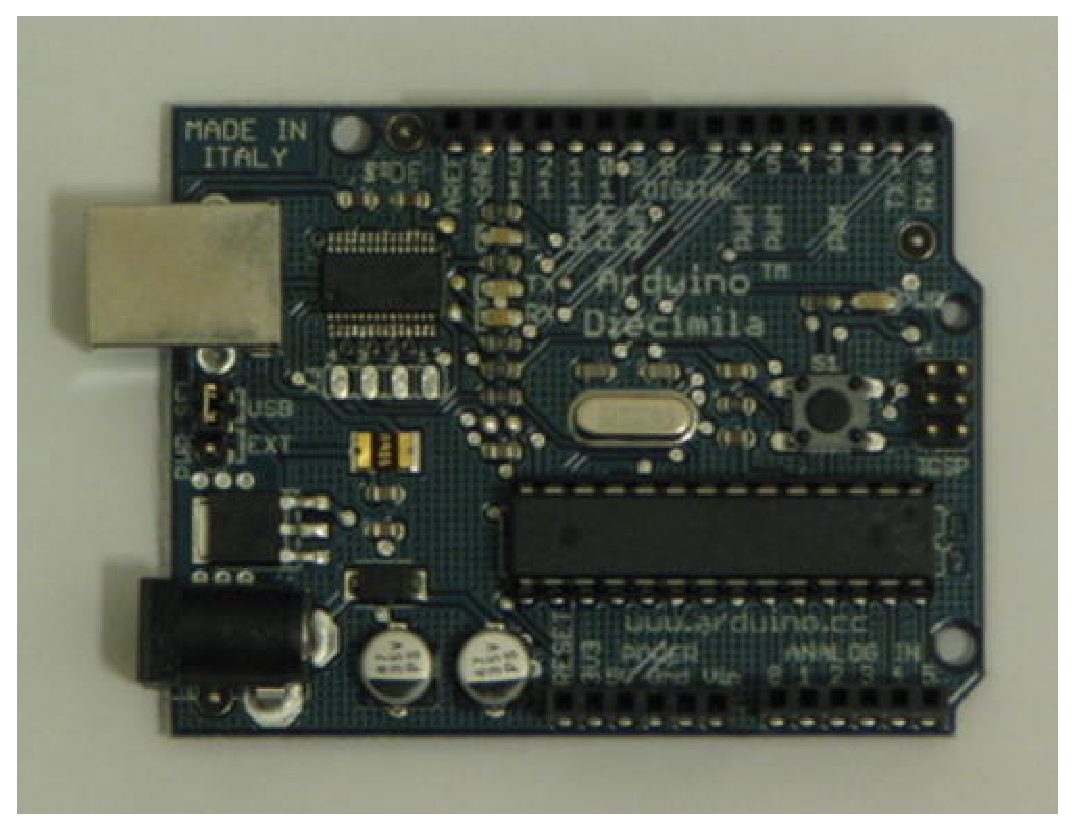
\includegraphics[scale = 0.5]{./figs/arduino.eps} % <- formatos PNG, JPG e PDF
	\caption[Foto do Arduino Diecimila]{Arduino Diecimila.}
	\fonte{http://blog.makezine.com/archive/2007/10/arduino \_ diecimila \_ and \_ bt.html}
	\label{fig:arduino}
\end{figure}

Os principais aspectos do Arduino que ser\~ao utilizados s\~ao a entrada/sa\'ida de dados e seu conversor D/A (digital para anal\'ogico) de 10 bits (01023), com a entrada de sinal anal\'ogico variando de um valor pr\'oximo de 0 V a um valor pr\'oximo de 5 V.

\subsection{Fio de N\'iquel-Cromo}

O fio de n\'iquel-cromo foi o tipo de fio utilizado como corda no projeto do instrumento. As caracter\'isticas que o material apresenta justificam essa escolha, baseando-se na sua utiliza\c{c}\~ao como resist\^encia el\'etrica. Optou-se pelo fio de espessura padr\~ao AWG 32, isto \'e, di\^ametro de aproximadamente 0,202 mm.

O n\'iquel-cromo ou simplesmente nicromo, \'e uma liga met\'alica composta por n\'iquel  majoritariamente  e cromo, e eventualmente ferro. Sua relativa alta resistividade e resist\^encia \`a oxida\c{c}\~ao em altas temperaturas fazem dessa liga uma op\c{c}\~ao muito utilizada na produ\c{c}\~ao de resist\^encias el\'etricas que tenham por fim produzir calor por efeito Joule, destinadas \`a utiliza\c{c}\~ao em aquecedores, secadores de cabelo, chocadeiras, seladoras de termopl\'astico, certos tipos de vela de igni\c{c}\~ao, entre outros. As propriedades esperadas do fio AWG 32 de nicromo seguem abaixo:

\begin{itemize}
\item Di\^ametro: $0,202 mm$;
\item Se\c{c}\~ao transversal: $0,0314 mm^{2}$;
\item Resist\^encia por metro: $34,6 \Omega/m$;
\item Densidade linear: $0,2625 g/m $;
\end{itemize}

Pretende-se utilizar cordas com comprimento aproximado de um metro, de forma que a resist\^encia m\'axima a ser aferida pelo sistema seja da ordem de algumas dezenas de ohms. O circuito de aferi\c{c}\~ao da resist\^encia foi projetado de forma que a tens\~ao aplicada sobre o fio seja da ordem de d\'ecimos de volt, garantindo que a intensidade da corrente el\'etrica no fio de valor adequado ao uso no projeto, ou seja, suficientemente pequeno para que a temperatura do fio seja segura para o usu\'ario.

\subsection{Potenci\^ometro}

O potenci\^ometro \'e um dispositivo eletr\^onico que funciona como um divisor de tens\~ao vari\'avel. Possui tr�s terminais, sendo dois deles fixos e um m\'ovel. Utilizando o terminal central com uma das extremidades \'e poss\'ivel utilizar esse dispositivo como um resistor vari\'avel. Nos modelos comuns, como apresentado na figura \ref{fig:potenciometro}, o ajuste \'e feito pelo movimento do eixo m\'ovel exposto, cuja varia\c{c}\~ao na maioria das vezes n\~ao ultrapassa 270. J\'a nos trimpots o ajuste \'e feito atrav\'es do movimento de um parafuso, somente acess\'ivel com o uso de uma chave de fenda. 

\begin{figure}[!htb]
	\centering
	\includegraphics[scale = 0.2]{./figs/potenciometro.eps} % <- formatos PNG, JPG e PDF
	\caption[potenci\^ometro]{Potenci\^ometro de 3/4 de volta.}
	\fonte{http://greduino.co.cc/wp-content/uploads/2009/09/Potentiometer.jpg}
	\label{fig:potenciometro}
\end{figure}

No projeto fez-se uso de trimpots multivoltas, cujo eixo realiza algumas voltas completas entre a posi\c{c}\~ao de resist\^encia m\'inima e a de m\'axima, devido \`a precis\~ao e confiabilidade requeridas. Eles s\~ao utilizados como os resistores de valores conhecido na ponte de Wheatstone, ajustados para exatamente o valor m\'aximo de resist\^encia do fio de n\'iquel-cromo utilizado. Al\'em disso, s\~ao utilizados para ajustar com precis\~ao o ganho dos amplificadores operacionais, para que nem subutilizem e nem ultrapassem a tens\~ao m\'axima de entrada do Arduino, que \'e de 5V.

\subsection{Ponte de Wheatstone}

De in\'icio, para a constru\c{c}\~ao do instrumento, decidiu-se utilizar uma ponte de Wheatstone, conforme mostrada na figura~\ref{fig:ponte}.

\begin{figure}[!htb]
	\centering
	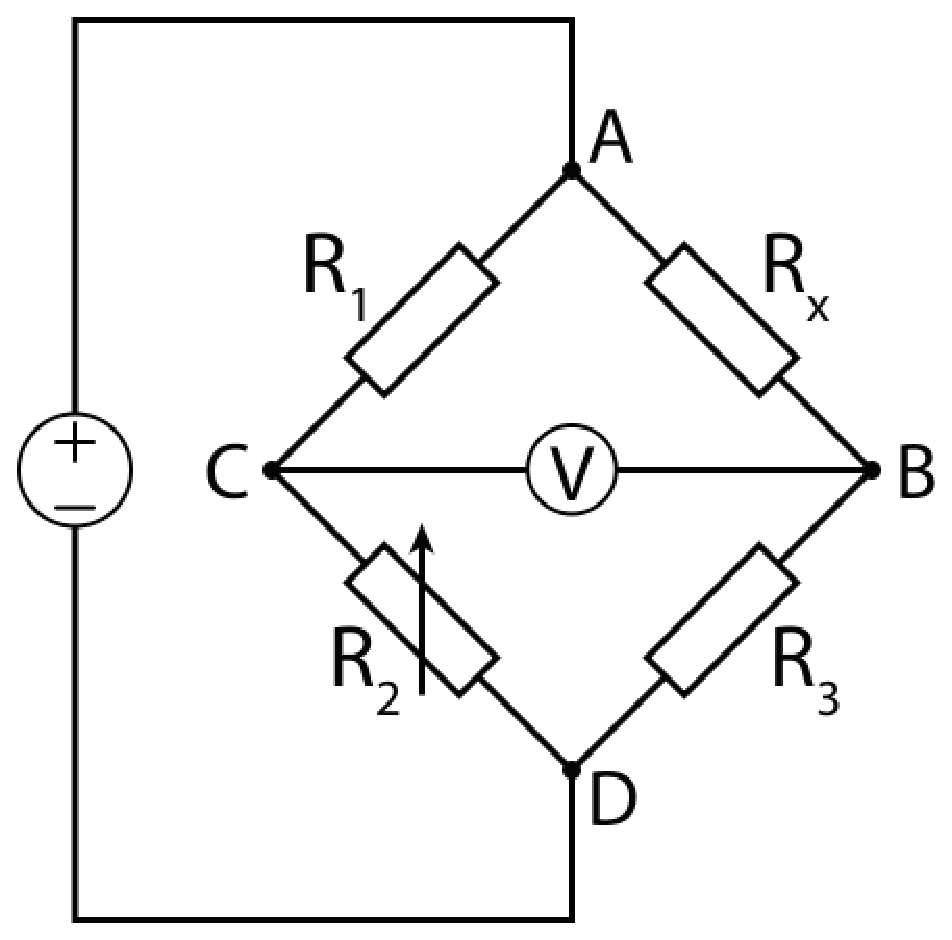
\includegraphics[scale = 0.5]{./figs/ponte.eps} % <- formatos PNG, JPG e PDF
	\caption[ponte de Wheastone]{Ponte de Wheatstone.}
	\fonte{http://pt.wikipedia.org/wiki/Ponte\_ de \_ Wheatstone}
	\label{fig:ponte}
\end{figure}

Esse circuito permite determinar o valor de uma resist\^encia desconhecida a partir de um arranjo com outras tr\^es resist\^encias de valor conhecido. A rela\c{c}\~ao entre as resist\^encias que caracteriza essa ponte \'e dada pela equa\c{c}\~ao 2.

\begin{equation}
R_1 R_3 = R_x R_2
\end{equation}

Contudo, essa rela\c{c}\~ao s\'o vale quando $V_{cb}$ \'e igual a $0$, o que n\~ao ocorre na maior parte do tempo, j\'a que a resist\^encia $R_x$ \'e vari\'avel. Logo, o que se mede com o circuito \'e justamente $V_{cb}$, visto que \'e dif\'icil projetar um resistor vari\'avel no lugar de $R_2$ que se ajustasse a todo momento para fazer valer a rela\c{c}\~ao matem\'atica da ponte. Com tr\^es resistores com valores iguais em $R_1$, $R_2$ e $R_3$ com valor semelhante ao m\'aximo do resistor desconhecido, $V_{cb}$ s\'o variar\'a entre 0 e $V_{ad}$. Contudo, variava de forma n\~ao-linear, e o c\'alculo de $R_x$ ent\~ao tornava-se impreciso, principalmente devido \`a instabilidade da ponte, que se mostrou inconveniente na hora de se confeccionar e manipular o circuito.

Por esses motivos, descartou-se esse m\'etodo de medi\c{c}\~ao da resist\^encia do fio. Em lugar da ponte de Wheatstone, utilizou-se uma solu\c{c}\~ao mais simples e elegante, que \'e o de calcular a resist\^encia utilizando-se as propriedades do ganho de um amplificador no circuito.

\subsection{Amplificador Operacional}

O amplificador operacional (amp-op) \'e um circuito integrado de complexidade relativamente alta que possui principalmente uma elevada quantidade de transistores interligados, o que por si s\'o j\'a significa uma dificuldade para compreender plenamente seu funcionamento atualmente e por isso a preocupa\c{c}\~ao nesse momento \'e utiliz\'a-lo corretamente de acordo com a necessidade. De acordo com Millman (1981), o amplificador operacional tem aplica\c{c}\~oes interessantes como amplificador de tens\~ao, amplificador de corrente, diferenciador, integrador, entre outras. O interesse \'e utiliz\'a-lo principalmente como amplificador de tens\~ao, na configura\c{c}\~ao amplificador n\~ao-inversor, apresentado pela figura~\ref{figampop}.

\begin{figure}[!htb]
	\centering
	\includegraphics[scale = 0.75]{./figs/ampop.eps} % <- formatos PNG, JPG e PDF
	\caption[Amplificador Operacional]{Amplificador Operacional, na configura\c{c}\~ao amplificador n\~ao-inversor.}
	\fonte{http://www.ifi.unicamp.br/~kleinke/f540/e \_ amp1.htm \# Nao \% 20inversor}
	\label{figampop}
\end{figure}

Nessa configura\c{c}\~ao, o ganho na sa\'ida \'e dado pela equa\c{c}\~ao 3.

\begin{equation}
G = {{V_out}/{V_inp}} = 1+ {{R_2}/{R_1}}
\end{equation}

Como exemplo, para se ter um ganho de 15 vezes \'e necess\'ario utilizar qualquer configura\c{c}\~ao de resistores em que $R_2$ tenha resist\^encia 14 vezes maior do que $R_1$. 

Para que o amplificador funcione como desejado \'e necess\'ario que a alimenta\c{c}\~ao seja no m\'inimo duas vezes superior \`a tens\~ao do sinal de sa\'ida. O amp-op utilizado no projeto \'e o LM324N, que tem quatro amplificadores operacionais no seu encapsulamento.


\subsection{Diagrama e Componentes do Circuito de Leitura}

O circuito apresentado na figura 6 \'e o utilizado para a leitura do valor de resist\^encia dos fios de nicromo. Partindo-se de uma fonte de 5 V, faz-se uso de um diodo comum para que a tens\~ao sobre o fio de nicromo seja constante e aproximadamente igual a 0,7 V, devido \`a queda de tens\~ao na jun\c{c}\~ao do diodo quando polarizado diretamente. Isso deve ser feito porque a liga de nicromo tende a elevar a sua temperatura quando sujeita \`a passagem de altas correntes, situa\c{c}\~ao em que dissipa elevada pot\^encia por efeito Joule. Al\'em disso, n\~ao se deseja a passagem de uma corrente elevada em um circuito que ser\'a diretamente utilizado pelo usu\'ario, pela sua pr\'opria seguran\c{c}a. Uma fotografia do circuito \'e exibida na figura~\ref{fig:fotocircuito}.

\begin{figure}[!htb]
	\centering
	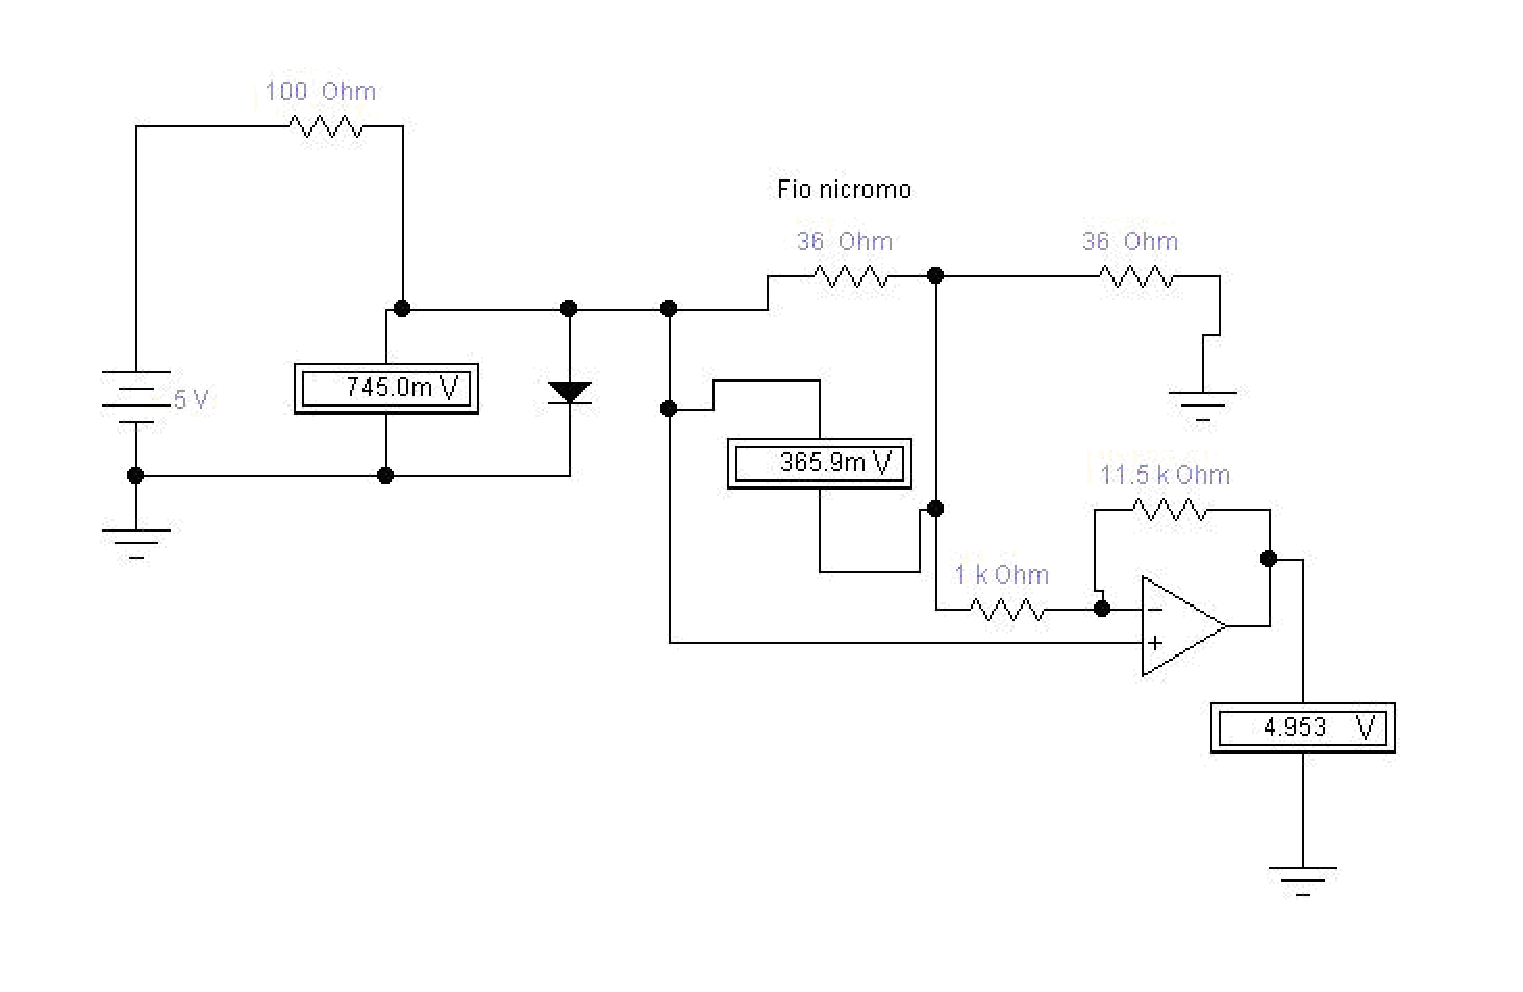
\includegraphics[scale = 0.5]{./figs/circuito.eps} % <- formatos PNG, JPG e PDF
	\caption[Esquema do Circuito de leitura]{Diagrama do Circuito de leitura de resist\^encia do fio de nicromo.}
	\fonte{Autoria Pr\'opria}
	\label{fig:circuito}
\end{figure}

\begin{figure}[!htb]
	\centering
	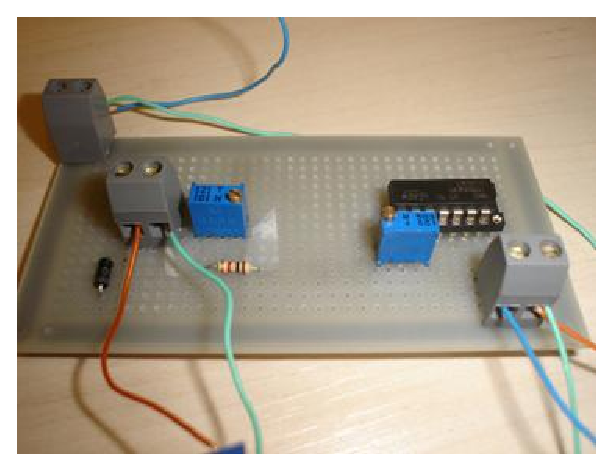
\includegraphics[scale = 0.75]{./figs/fotocircuito.eps} % <- formatos PNG, JPG e PDF
	\caption[Foto do Circuito de leitura]{Foto do Circuito de leitura de resist\^encia do fio de nicromo.}
	\fonte{Autoria Pr\'opria}
	\label{fig:fotocircuito}
\end{figure}

A resist\^encia de 100 ohms no terminal da fonte \'e utilizada para garantir a tens\~ao m\'inima de condu\c{c}\~ao no diodo, permitindo a passagem de um valor baixo de corrente, suficiente para a amplifica\c{c}\~ao do amp-op ao mesmo tempo que n\~ao  apresenta riscos de superaquecimento do fio. J\'a a resist\^encia de 36 ohms \'e apenas um divisor de tens\~ao de valor aproximadamente igual ao da resist\^encia m\'axima do fio, assim escolhida para fixar um intervalo conveniente de valores da tens\~ao sobre o fio de nicromo.

A tens\~ao nos pontos em que est\'a ligado o amp-op \'e a pr\'opria tens\~ao sobre o fio de nicromo e varia, portanto, aproximadamente de 0 a 0,35 V. O amp-op \'e utilizado para que seja poss\'ivel a obten\c{c}\~ao de maior sensibilidade do circuito em rela\c{c}\~ao \`a varia\c{c}\~ao de resist\^encia do fio, ao impor um ganho sobre a tens\~ao de sa\'ida. Ao alargar a faixa de valores dessa tens\~ao, \'e poss\'ivel ent\~ao se obter valores satisfat\'orios na convers\~ao de anal\'ogica para digital. O circuito amplificador utilizado tem um ganho aproximado entre 13 a 14 vezes. Alimentando esse circuito com as sa\'idas da fonte de 5 V e o amp-op com as de 12 V, os valores nominais aferidos pelo kit com microcontrolador pouco ultrapassam os 4,25 V. Um ganho maior n\~ao \'e desej\'avel; por exemplo,  utilizando-se um ganho de 15 vezes, a tens\~ao de pico chega a aproximados 4,85 V, o que ultrapassa o limite superior de funcionamento do conversor A/D, de tal forma que a medi\c{c}\~ao de um certo intervalo de valores da resist\^encia acabam sendo cortada.

\section{Circuito de Detec\c{c}\~ao de Obstru\c{c}\~ao (toque da corda do instrumento}

Em adi\c{c}\~ao \`a aferi\c{c}\~ao da tonalidade em que se sup\~oe que a corda do instrumento vibrasse, \'e necess\'ario que o sistema possa reconhecer o instante em que o usu\'ario toca uma nota, ``beliscando'' determinada corda. Para isso, adotou-se um sensor de presen\c{c}a como representando cada corda, de tal forma que, quando o usu\'ario deseja tocar uma nota, ele deve simplesmente obstruir o respectivo sensor com os dedos.

Idealizou-se esse detector de obstru\c{c}\~ao com o uso de LEDs infravermelhos e fotodiodos, numa abordagem baseada no projeto de Oficinas de Integra\c{c}\~ao 1, ``Sistema de aquisi\c{c}\~ao e tratamento de dados para experi\^encias de cinem\'atica''. A partir do momento em que haja uma obstru\c{c}\~ao da recep\c{c}\~ao de luz infravermelha do fotodiodo, deixar\'a de haver condu\c{c}\~ao e consequentemente \'e poss\'ivel ler um n\'ivel l\'ogico baixo. Caso contr\'ario, ou seja, na situa\c{c}\~ao normal em que h\'a recep\c{c}\~ao e emiss\~ao de luz infravermelha, a leitura \'e de um sinal com n\'ivel l\'ogico alto. Essas respostas \`as duas situa\c{c}\~oes, explicadas na se\c{c}\~ao~\ref{subsec:LED}, fazem o sensor ser capaz de detectar a presen\c{c}a de um objeto qualquer posicionado entre o LED infravermelho e o fotodiodo.

\subsection{LED Infravermelho e Fotodiodo}
\label{subsec:LED}

Os diodos s\~ao compostos por uma jun\c{c}\~ao PN, isto \'e, uma composi\c{c}\~ao de dois tipos de semicondutores, P e N, que s\~ao classificados de acordo com a natureza da dopagem existente em sua composi\c{c}\~ao. A parte de tipo N \'e feita pela dopagem de elementos qu\'imicos pentavalentes, como o antim\^onio e o f\'osforo, cujos el\'etrons livres em excesso conferem a eles uma grande tend\^encia de doar el\'etrons. A de tipo P por sua vez, \'e feita pela dopagem de impurezas trivalentes, como o \'indio e o alum\'inio, e apresentam grande tend\^encia a aceitar el\'etrons, pelo predom\'inio de lacunas. Os portadores de carga majorit\'arios no semicondutor tipo P e no tipo N s\~ao, respectivamente, el\'etrons e lacunas.

A jun\c{c}\~ao desses dois tipos de semicondutor gera a chamada zona de deple\c{c}\~ao, que surge pela tend\^encia dos portadores de carga de cada um dos semicondutores de migrar para o outro, recombinando-se, um el\'etron com uma lacuna. Com isso, uma concentra\c{c}\~ao de \'ions ocorre na regi\~ao pr\'oxima \`a jun\c{c}\~ao, pois cada semicondutor passa a ter excesso de cargas ap\'os a sua migra\c{c}\~ao.

\'E devido a essa zona de deple\c{c}\~ao que o diodo apresenta seu comportamento t\'ipico. Se ligado na polaridade direta, e a tens\~ao for suficiente para vencer o potencial da zona de deple\c{c}\~ao, desalojando os \'ions e criando portadores de carga livres novamente, ele conduz corrente. Se ligado na polaridade reversa, n\~ao passa corrente pelo diodo, pois a polariza\c{c}\~ao do campo el\'etrico aumenta ainda mais a largura da zona de deple\c{c}\~ao, ao promover a migra\c{c}\~ao de mais portadores de carga entre os dois tipos de semicondutor. 

Quando um el\'etron retorna da banda de condu\c{c}\~ao para a banda de val\^encia, ele eventualmente encontra uma lacuna, e elimina-se a exist\^encia de um par lacuna-el\'etron, fen\^omeno chamado de recombina\c{c}\~ao. Na recombina\c{c}\~ao em semicondutores, a energia liberada \'e transferida para a estrutura cristalina na forma de calor. Entretanto, alguns semicondutores, como o feito a partir arseneto de g\'alio, que apresentam altos \'indices de recombina\c{c}\~ao, a libera\c{c}\~ao de energia ocorre na forma de radia\c{c}\~ao, parcialmente luz vis\'ivel e na maior parte luz infravermelha. A maior libera\c{c}\~ao de luz acontece pr\'oxima \`a jun\c{c}\~ao PN, que \'e onde ocorre a maior parte das recombina\c{c}\~oes. O LED infravermelho emite radia\c{c}\~ao eletromagn\'etica no espectro infravermelho, que n\~ao \'e vis\'ivel ao olho humano.

O fotodiodo, por sua vez, \'e basicamente um diodo com inv\'olucro transparente sobre a jun\c{c}\~ao PN. Esse diodo age como fotodetector, por responder a uma entrada em forma de luz. Pode ser utilizado em duas configura\c{c}\~oes, na polariza\c{c}\~ao direta ou inversa. Na primeira, a incid\^encia de radia\c{c}\~ao em certas faixas de frequ\^encia sobre o fotodiodo, espec\'ificas para cada material do qual ele \'e feito, faz com que se produza sobre ele uma corrente e uma tens\~ao espec\'ificas, dependendo do modo de opera\c{c}\~ao. J\'a na polariza\c{c}\~ao inversa, o fotodiodo apresenta elevada resist\^encia \`a passagem de corrente, que diminui com a incid\^encia de luz. Monitorando-se essa mudan\c{c}a, o fotodiodo em polariza\c{c}\~ao reversa pode ser usado como detector da presen\c{c}a de luz.

\section{Fonte de Alimenta\c{c}\~ao}

Circuitos que realizam amplifica\c{c}\~ao de sinal, como circuitos que cont\'em amplificadores operacionais, s\~ao bastante sens\'iveis a mudan\c{c}as na alimenta\c{c}\~ao. Uma bateria comum de 9 V, por exemplo, tornaria o circuito impreciso, pois ao perder carga apresenta
 flutua\c{c}\~oes na tens\~ao fornecida. No caso do circuito de leitura anal\'ogica, ocorreria uma altera\c{c}\~ao dos valores extremos de leitura m\'axima, causando efeitos indesejados na leitura, como a recep\c{c}\~ao de uma faixa de dados cada vez menor. 

Como o circuito de leitura da resist\^encia do fio de nicromo requer precis\~ao e n\~ao admite perda de sensibilidade ao longo do tempo, optou-se por construir uma fonte de alimenta\c{c}\~ao de corrente cont\'inua, a ser utilizada sempre que o circuito venha a necessitar de alimenta\c{c}\~ao, incluindo-se nessa situa\c{c}\~ao o kit de microcontrolador Arduino. A fonte \'e apresentada na figura~\ref{fig:fonte}.

\begin{figure}[!htb]
	\centering
	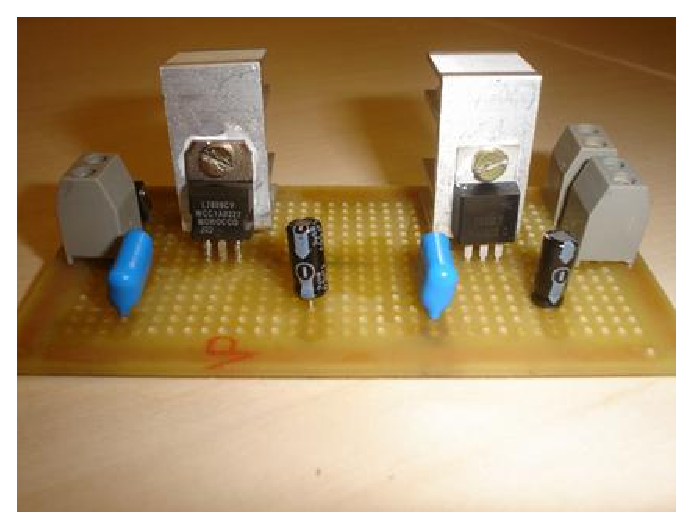
\includegraphics[scale = 0.75]{./figs/fonte.eps} % <- formatos PNG, JPG e PDF
	\caption[Foto da Fonte]{Fonte de alimenta\c{c}\~ao.}
	\fonte{Autoria Pr\'opria}
	\label{fig:fonte}
\end{figure}

Na pr\'atica, a fonte n\~ao chega a ser um conversor AC/DC completo, mas sim um adaptador DC/DC que, a partir de uma fonte de 12 V /1 A, gera tens\~oes de sa\'ida de 12 V, 9 V e 5 V, para alimentar, respectivamente, o amplificador operacional, o Arduino e o circuito de leitura respectivamente. Os principais componentes do circuito do circuito s\~ao os reguladores de tens\~ao LM7809 e LM7805, al\'em de capacitores de $0,33 \mu F$ e $1 \mu F$.

\chapter{Software}

\section{Biblioteca de fun\c{c}\~oes}

O hardware, atrav\'es da plataforma Arduino, comunica-se com o computador usando a porta serial. A porta serial utilizada \'e uma porta USB (normalmente com conector USB-A). O driver USB utilizado, FTDI, simula o funcionamento de uma porta COM, criando uma porta COM virtual; ou seja, apesar de usar-se uma porta USB para a comunica\c{c}\~ao serial, v\^e-se, do ponto de vista do software, uma porta COM (RS 232).

Para essa comunica\c{c}\~ao, foi desenvolvida uma biblioteca de fun\c{c}\~oes em linguagem C++, com o objetivo de permitir, de forma encapsulada, o envio de informa\c{c}\~oes para o hardware e o recebimento de informa\c{c}\~oes dele. A biblioteca funciona como uma interface entre a aplica\c{c}\~ao pr\'atica (alto n\'ivel) com a comunica\c{c}\~ao serial e o protocolo de envio (baixo n\'ivel), conforme esquematizado na figura~\ref{fig:biblioteca}. A documenta\c{c}\~ao da biblioteca est\'a apresentada no ap\^endice A. A comunica\c{c}\~ao \'e baseada no recebimento de pedidos e envio de respostas, ou seja, o hardware s\'o envia informa\c{c}\~oes para o computador quando, de alguma forma, requisita-se que ele as envie. Tal mecanismo apresenta a vantagem de o computador n\~ao ter de ficar constantemente recebendo e processando dados da porta serial, e tamb\'em permite uma maior facilidade de distin\c{c}\~ao da natureza das informa\c{c}\~oes recebidas.

\begin{figure}[!htb]
	\centering
	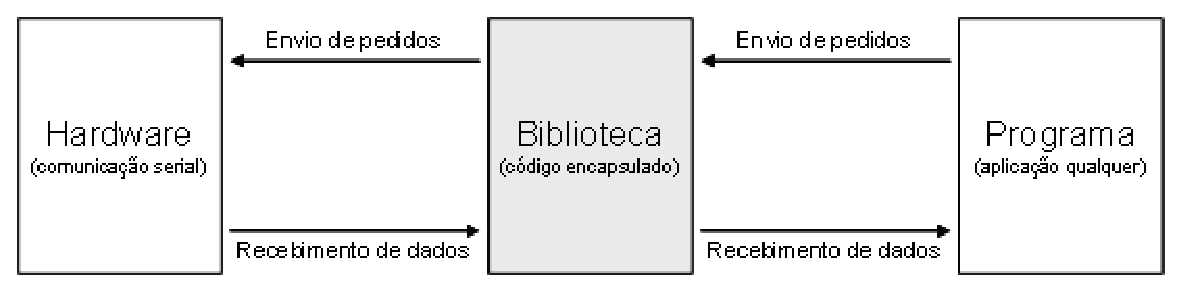
\includegraphics[scale = 0.75]{./figs/comunicacaosoftware.eps} % <- formatos PNG, JPG e PDF
	\caption[Comunica\c{c}\~ao do Software]{Diagrama ilustrativo do funcionamento da biblioteca.}
	\fonte{Autoria Pr\'opria}
	\label{fig:biblioteca}
\end{figure}


A maneira pela qual as informa\c{c}\~oes s\~ao enviadas e recebidas atrav\'es da porta serial foi elaborada de forma que fosse facilmente extens\'ivel, e que futuras extens\~oes mantivessem a compatibilidade reversa. As informa\c{c}\~oes s\~ao sempre acompanhadas de algo que identifica sua natureza, o que, apesar de redundante na maioria dos casos, ajuda a evitar erros.

O c\'odigo da biblioteca \'e exclusivo para sistema operacional Windows, visto que utiliza fun\c{c}\~oes nativas desse sistema operacional para comunicar-se com a porta serial. Por\'em, pequenas adapta\c{c}\~oes no c\'odigo permitiriam portar o c\'odigo para sistemas baseados em UNIX.

\section{Comunica\c{c}\~ao com o hardware}

A comunica\c{c}\~ao serial atrav\'es de uma porta COM pode ser entendida como um fluxo de bits (do ingl\^es, bitstream). Tanto a biblioteca quanto o hardware entendem os bytes como caracteres de acordo com a codifica\c{c}\~ao ASCII. A menor unidade de informa\c{c}\~ao que a biblioteca troca com o hardware \'e chamada de ``mensagem''. As mensagens s\~ao sequ\^encias de caracteres invariavelmente terminadas pelos caracteres de \emph{carriage return} e \emph{line feed}, representados pelos c\'odigos 13 e 10.

Uma mensagem \'e formada por uma instru\c{c}\~ao e, se necess\'ario, um ou mais par\^ametros. O que divide uma instru\c{c}\~ao de seus par\^ametros, e os par\^ametros entre si, s\~ao caracteres de espa\c{c}o, representados pelo c\'odigos 32. No conte\'udo dos par\^ametros tamb\'em podem existir caracteres de espa\c{c}o.

Cada par\^ametro tem um nome e um valor, separados entre si por um sinal de igual, representado pelo c\'odigos 61. Entre o nome de um par\^ametro, o sinal de igual e o seu valor podem existir um ou mais espa\c{c}os. O valor dos par\^ametros \'e representado por uma cadeia de caracteres circundados por aspas duplas. Para inserir as aspas duplas no valor de algum par\^ametro, usa-se o caractere barra invertida (``\textbackslash '') seguida das aspas duplas. De forma similar, para indicar a barra invertida, usa-se um par de caracteres de barra invertida.

Por conveni\^encia, convencionou-se que as instru\c{c}\~oes e par\^ametros s\~ao identificados por palavras ou mnem\^onicos em l\'ingua inglesa, visto que a tabela ASCII padr\~ao n\~ao apresenta caracteres espec\'ificos do alfabeto da l\'ingua portuguesa, como os acentos, a cedilha ou o til. Uma tabela com as instru\c{c}\~oes trocadas pela biblioteca e pelo hardware, acompanhados de seus respectivos par\^ametros, \'e apresentada no ap\^endice A.

\chapter{Considera\c{c}\~oes Finais}

\section {Or\c{c}amento}
\begin{table}[!htb]
	\centering
	\caption[Or\c{c}amento do Projeto]{Tabela de custos dos componentes utilizados no projeto}
	\label{tab:orcamento}
	\begin{tabular}{cccc}

\hline
Componente/produto & Valor unit\'ario & Unidades & Valor \\
\hline
Folha de foam n\~ao revestido(A0) & R\$12,90 & 1 & R\$12,90 \\
Fio resistivo de nicromo (com frete) & R\$11,00 (m) + R\$8,00 & 5 & R\$63,00 \\
Arduino diecemila & R\$72,00 & 1 & R\$72,00 \\
Placa de circuito impresso universal & R\$3,00 & 3 & R\$9,00 \\
Resistores 1k &	R\$0,30 & 1 & R\$0,30 \\
Resistores 100 ohms & R\$ 0,40 & 1 & R\$0,40 \\
Capacitores 330k & R\$0,70 & 2 & R\$1,40 \\
Capacitores 1F & R\$ 0,60 & 2 & R\$ 1,20 \\
CI LM324N & R\$ 0,80 & 1	& R\$ 0,80 \\
Conectores & R\$0,40 & 8	& R\$3,20 \\
Trimpot de multivoltas (100k) & R\$ 2,00	& 2 & R\$4,00 \\
Reguladores & R\$ 1,80 & 2 & R\$3,60 \\
Outros (solda, pasta, cola de isopor...)* & & &	R\$3,00 \\
Outros(socket, plug, diodos...)* & & & R\$3,00 \\
Total & & & R\$177,80 \\
\hline
	\end{tabular}
	\fonte{Autoria pr\'opria.}
\end{table}

\section{Coment\'ario do Desenvolvimento do Projeto}

O instrumento como um coletor de dados est\'a quase totalmente implementado. O circuito de leitura do fio est\'a finalizado, assim como o software de comunica\c{c}\~ao com o computador, que recebe os dados lidos atrav\'es do Ardu\'ino. O circuito detector da obstru\c{c}\~ao, respons\'avel por sinalizar a vibra\c{c}\~ao das cordas, ainda n\~ao est\'a conclu\'ido.

Al\'em disso, embora n\~ao fosse objetivo prim\'ario do projeto, um programa que interpretasse as informa\c{c}\~oes recebidas pelo instrumento e a traduzisse em sons n\~ao foi desenvolvido. Contudo, devido \`a flexibilidade do protocolo utilizado no software de recebimento dos dados, isso seria facilmente implementado, n\~ao fossem as dificuldades inerentes ao aplicativo que se tentaria desenvolver.

\section{Potencialidades do Projeto}

Enfatiza-se aqui o fato de que o sistema, como um todo, foi projetado de modo a permitir mudan\c{c}as substanciais nas caracter\'isticas do instrumento f\'isico e da interface de interpreta\c{c}\~ao dos dados emitidos. Ou seja, as propriedades e tamb\'em a finalidade do sistema s\~ao flex\'iveis.

O projeto foi executado de forma a ser facilmente adapt\'avel posteriormente. Ser\'a poss\'ivel utiliz\'a-lo n\~ao apenas para a gera\c{c}\~ao de sons; jogos ou aplicativos gr\'aficos, instrumento de grava\c{c}\~ao de arquivos de \'audio ou ferramenta de aprendizado s\~ao algumas das finalidades nas quais o sistema poder\'a ser empregado.


%---------- Referencias ----------
\renewcommand{\ABNTbibliographyname}{REFER\^ENCIAS}
\bibliography{reflatex} % geracao automatica das referencias a partir do arquivo reflatex.bib

\chapter{Refer\^encias Bibliogr\'aficas}

\begin{list}{}{}

\item KLEINKE, Maurcio Urban. "Vis\~ao Introdu\c{c}\~ao a eletr\^onica e dispositivos semicondutores. Campinas, S\~ao Paulo. 2002. Disponvel em: <http://www.ifi.unicamp.br/~kleinke/f540/f540.htm> Acesso em 14.10.2009.

\item MILLMAN, Jabob; HALKIAS, Christos C. Eletr\^onica: Dispositivos e Circuitos. Vol. 2. McGraw Hill. 1981.

\item MEDIDAS de resist\^encia com a ponte de Wheatstone. Disponvel em: <http://www.fisica.ufsc.br/~lab2/pdfs/exp03.pdf> Acesso em 14.10.2009.

\item MACHADO, Bruno R. P.; SIMAS, Joo H. C.; GIOPPO, Lucas L. Sistema de Aquisi\c{c}\~ao de Dados para Experi\^encias de Cinem\'atica, Trabalho de Oficinas I, Engenharia de Computa\c{c}\~ao, UTFPR. Curitiba, 2008. 

\item SOMMERVILLE, Ian. Engenharia de Software, 8 edi\c{c}\~ao; tradu\c{c}\~ao: Selma Shin Shimizu Melnikoff, Reginaldo Arakkaki, Edlson de Andrade Barbosa. S\~ao Paulo, Pearson Addison Wesley, 2007. 

\end{list}




%---------- Apendices (opcionais) ----------
\apendice

\chapter{Documenta\c{c}\~ao da biblioteca de software.}

A biblioteca de comunica\c{c}\~ao com o instrumento atrav\'es da porta serial \'e composta primariamente da classe \emph{ConexaoInstrumento}, que define m\'etodos de alto n\'ivel diversos para obten\c{c}\~ao de dados a partir do instrumento. Tamb\'em comp\~oe a biblioteca a estrutura corda, capaz de armazenar o estado de uma corda do instrumento (tem dois atributos: \emph{posicao}, que indica a posi\c{c}\~ao em que est\'a o dedo, e soando, que indica se o sensor da corda est\'a ou n\~ao obstruido). Num aplicativo com programa\c{c}\~ao paralela (\emph{multithreading}), n\~ao \'e seguro que o objeto seja acessado simultaneamente por mais de uma linha de execu\c{c}\~ao (\emph{thread}).

\begin{figure}[!htb]
	\centering
	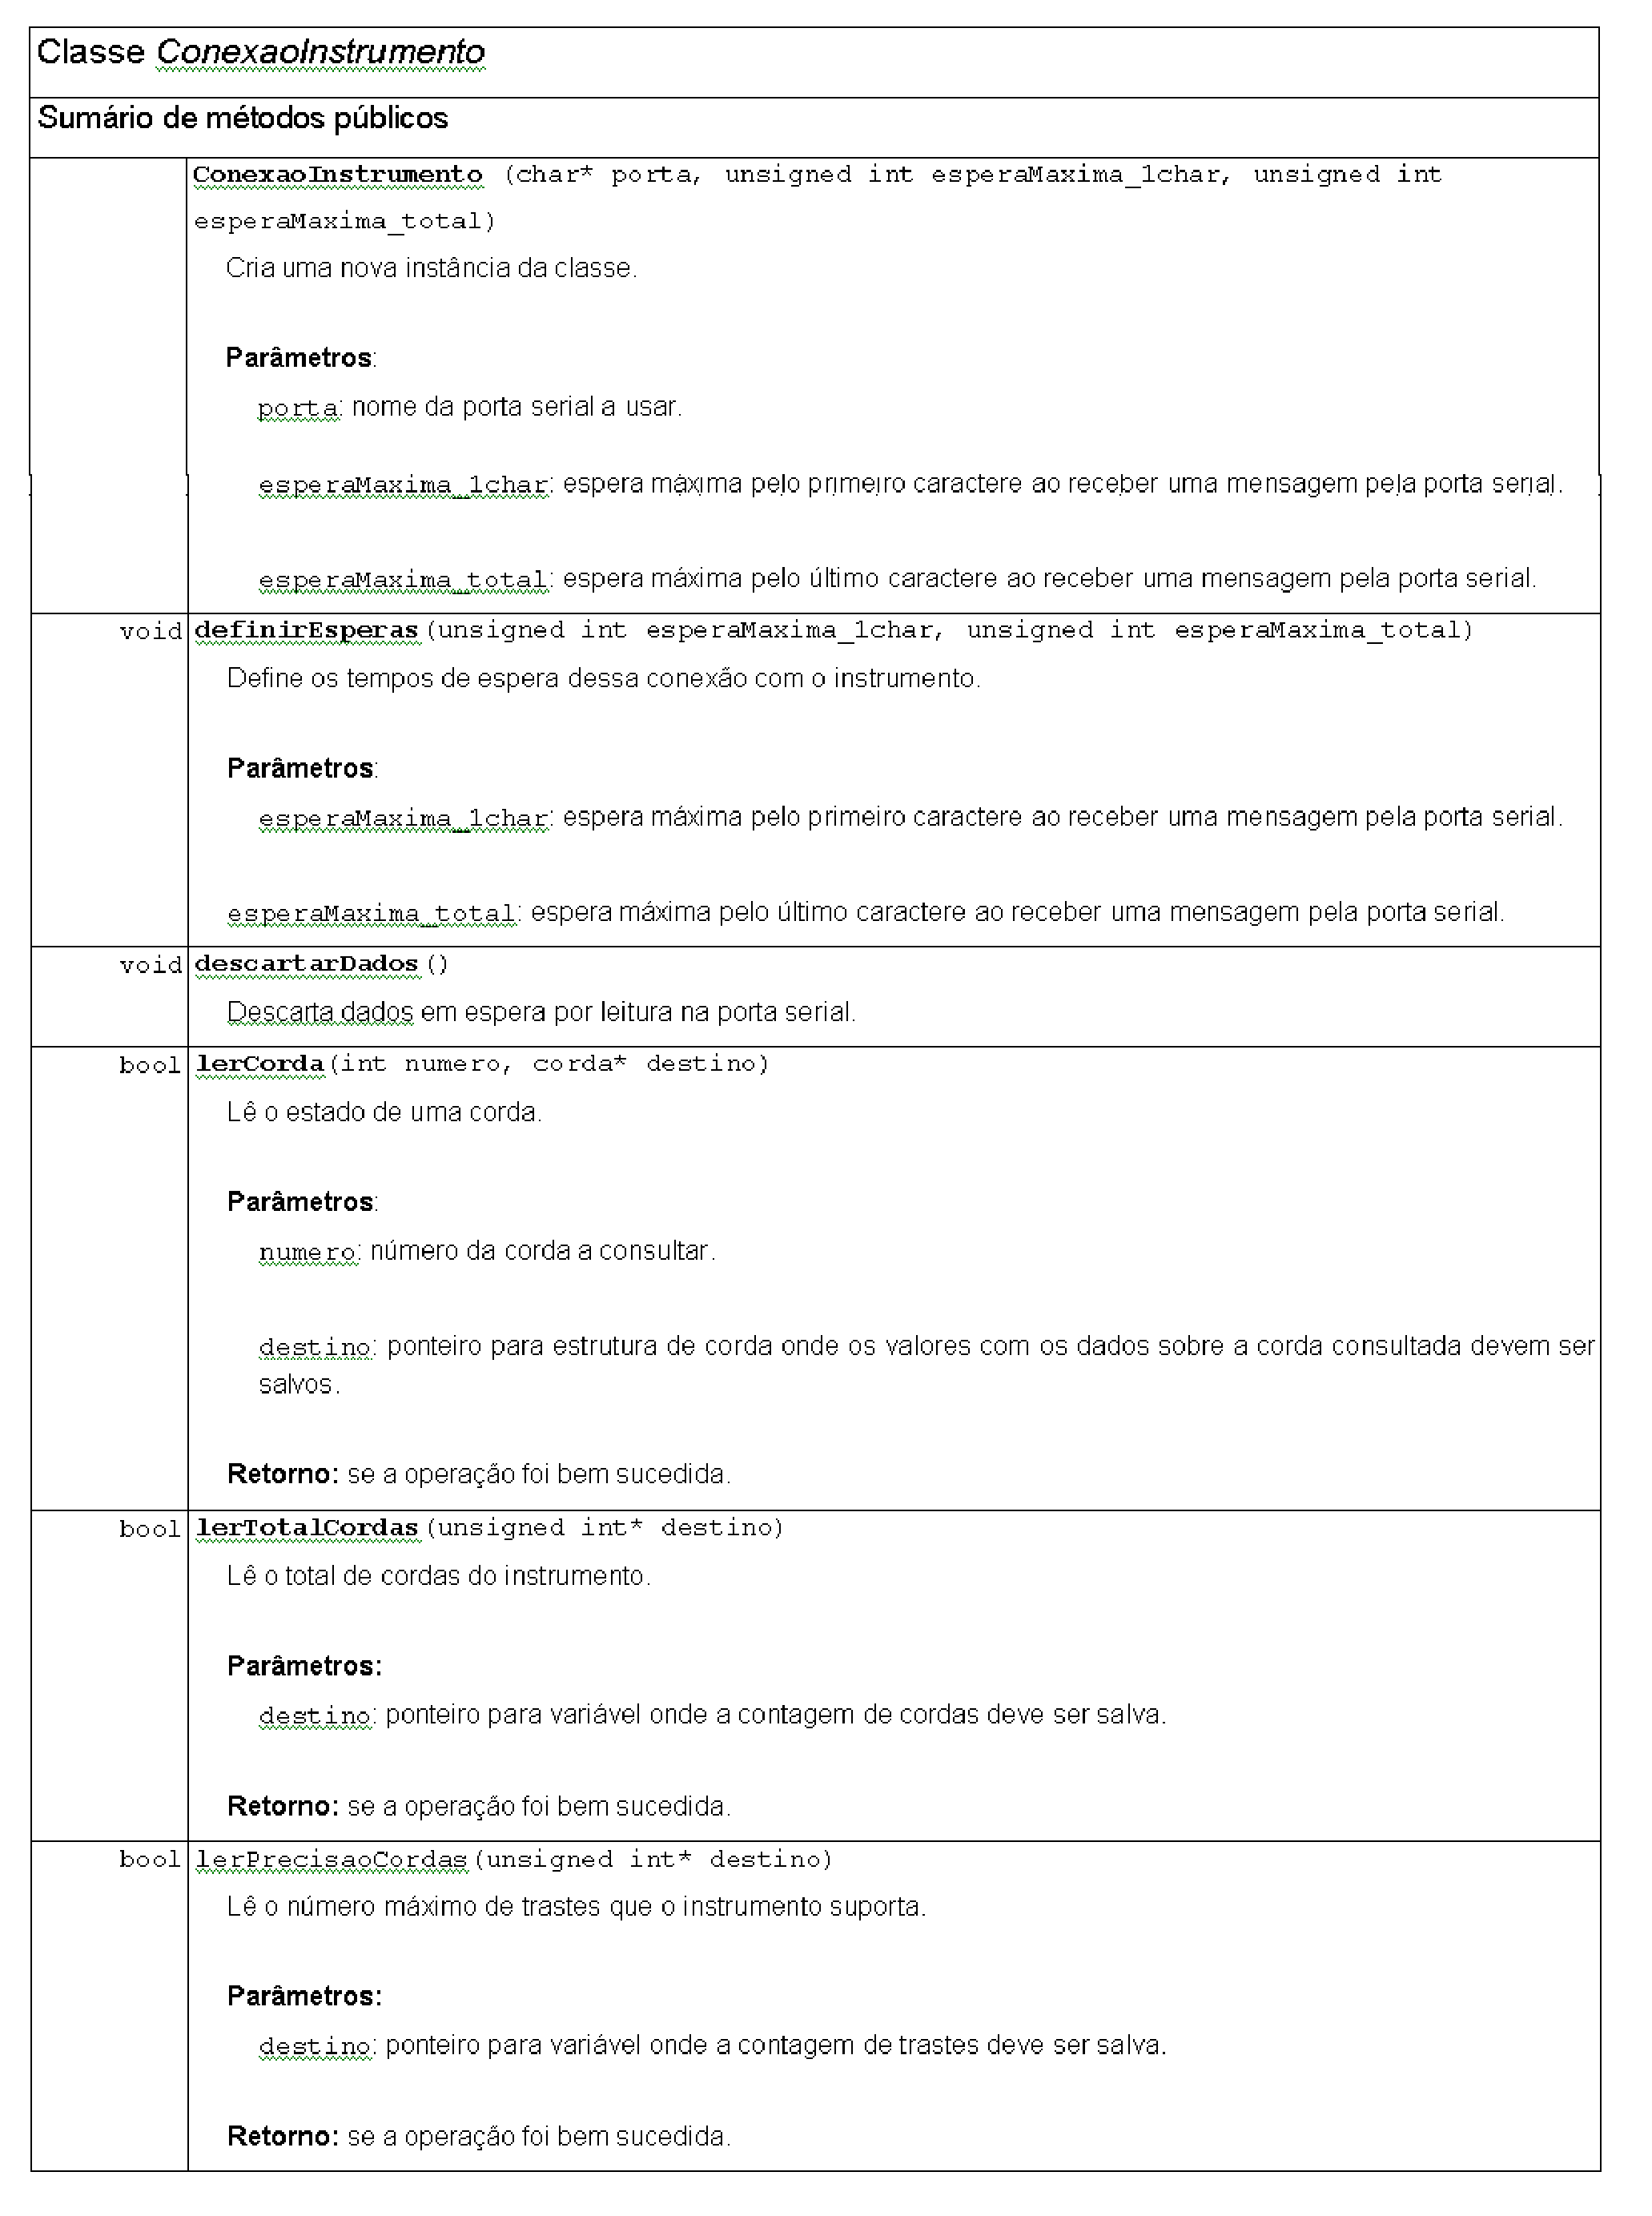
\includegraphics[scale = 0.45]{./figs/apendicea.eps} % <- formatos PNG, JPG e PDF
	\label{fig:apendicea}
\end{figure}

\chapter{Mensagens do sistema de comunica\c{c}\~ao.}

\begin{figure}[!htb]
	\centering
	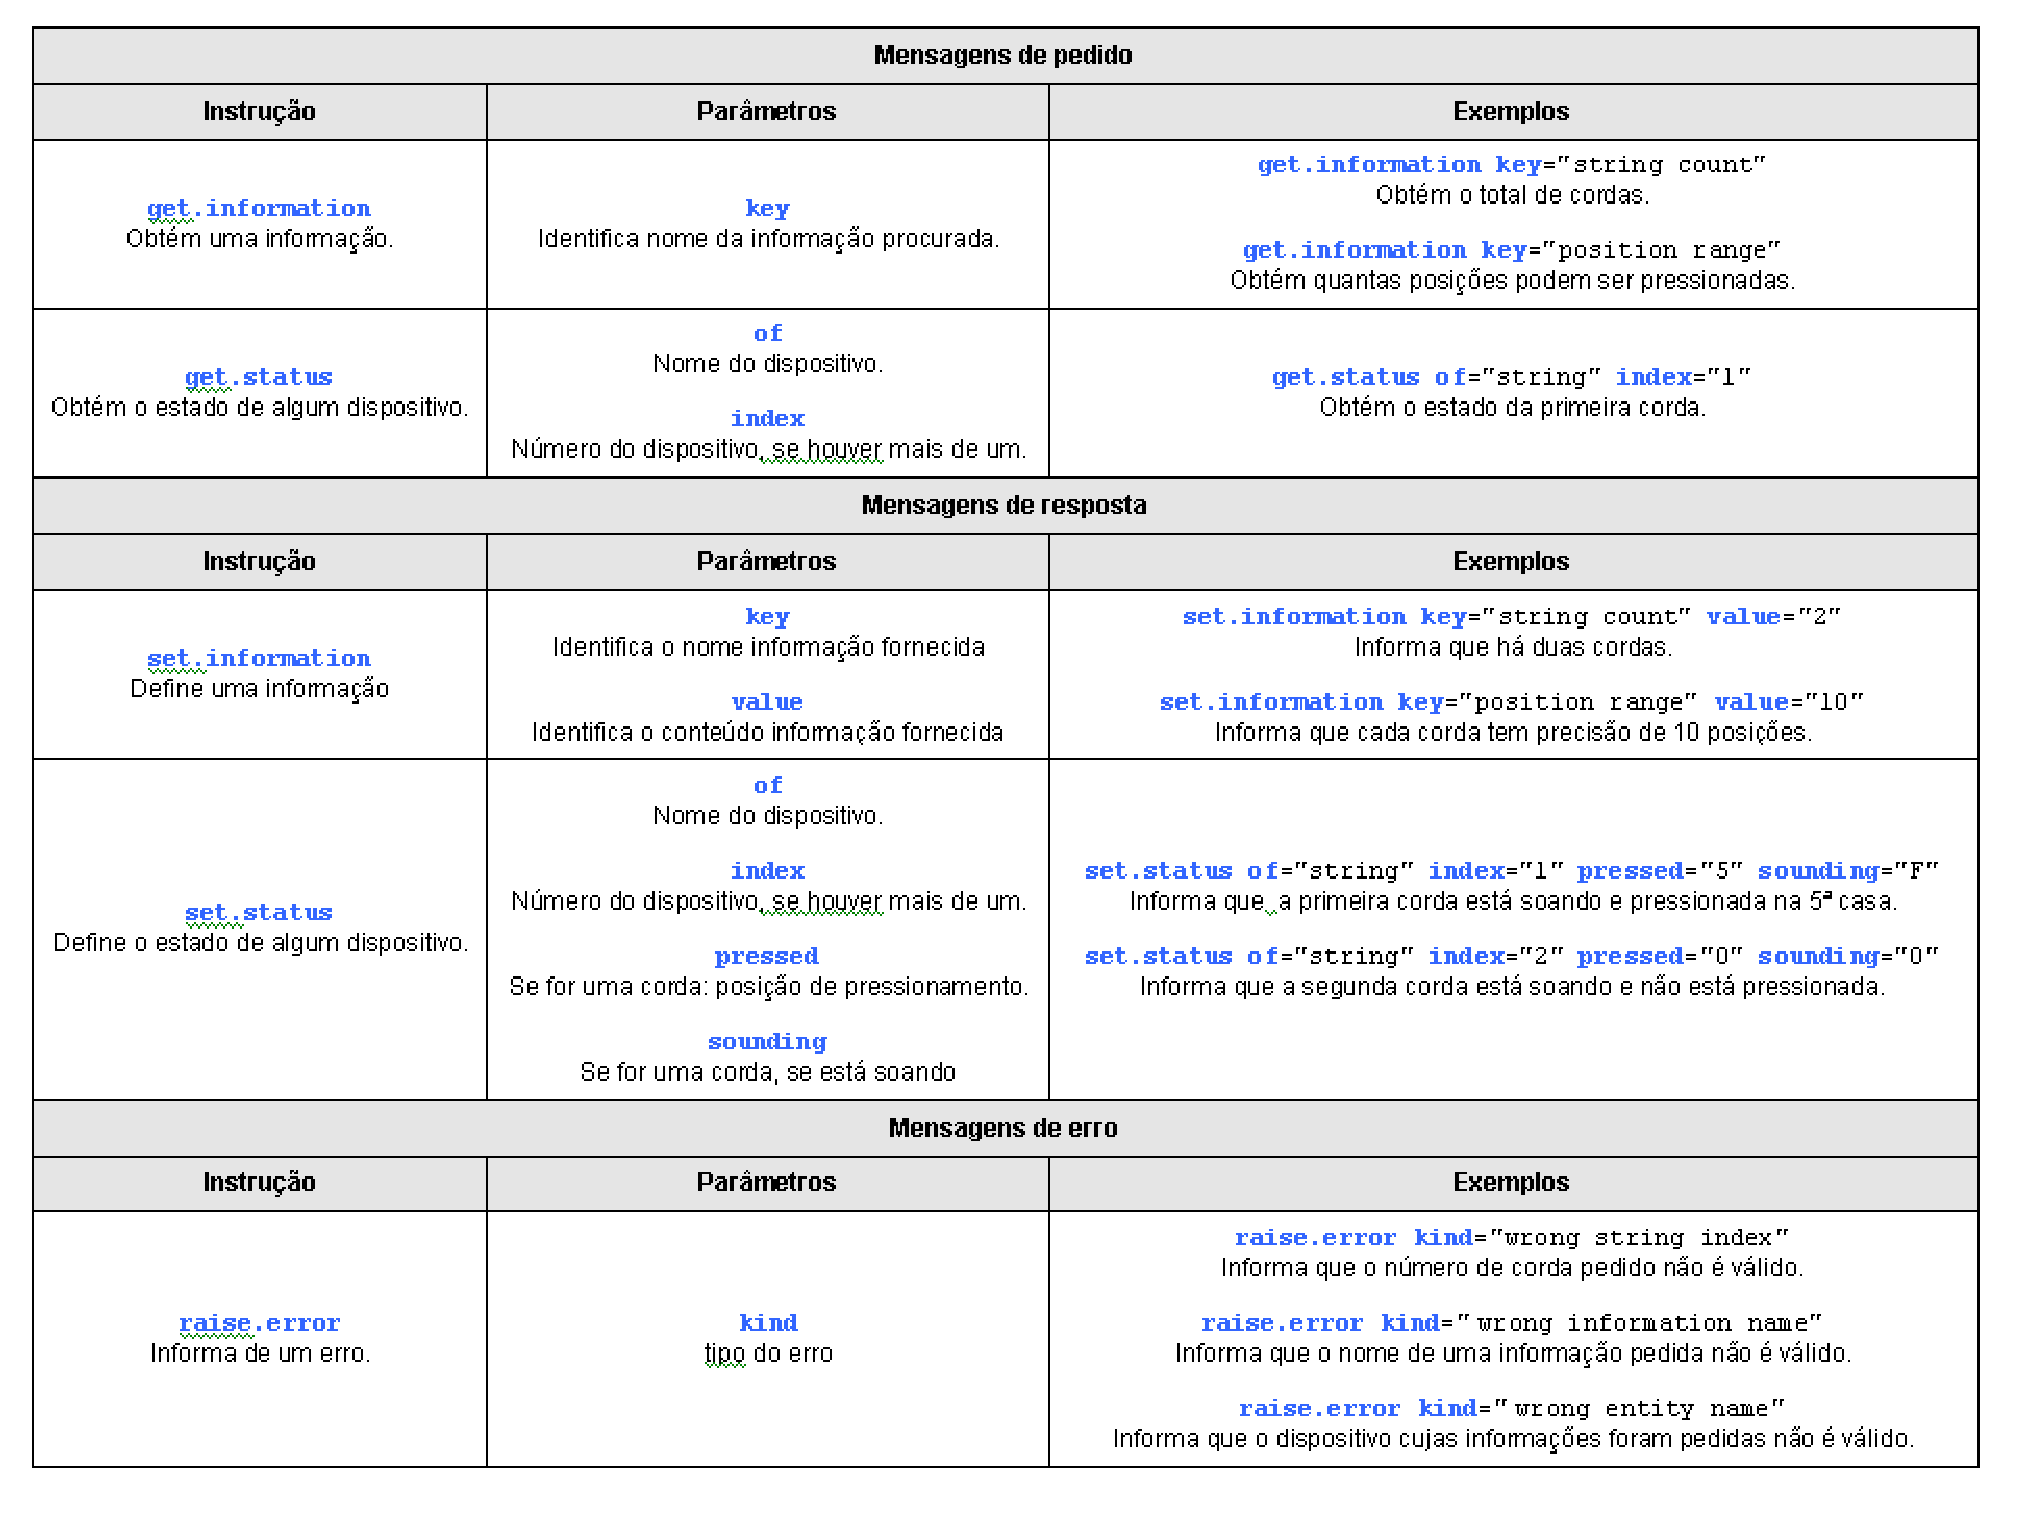
\includegraphics[scale = 0.45]{./figs/apendiceb.eps} % <- formatos PNG, JPG e PDF
	\label{fig:apendiceb}
\end{figure}

\end{document}


